%--------------------------------------------------------------------%
%
% Berkas utama templat Skripsi Universitas Negeri Malang.
%
% mengikuti Pedoman Penulisan Karya Ilmiah UM Edisi 2017.
%
%--------------------------------------------------------------------%

\documentclass[12pt, a4paper, onecolumn, oneside, final]{report}

\input{config/if-itb-thesis.sty}
%-------------------------------------------------------------------%
%
% Informasi umum skripsi — SUNTING DI SINI SAJA.
% Semua halaman front matter mengambil nilai dari makro di bawah.
%
%-------------------------------------------------------------------%

\newcommand{\judul}{Judul Skripsi yang Informatif dan Mencerminkan Isi}
\newcommand{\penulis}{Nama Lengkap Penulis}
\newcommand{\nim}{123456789}

\newcommand{\jurusan}{Jurusan Teknik Informatika}
\newcommand{\fakultas}{Fakultas Teknik}
\newcommand{\programstudi}{Program Studi Pendidikan Informatika}
% Diisi pada halaman judul: "...menyelesaikan program <gelarprogram>"
\newcommand{\gelarprogram}{Sarjana Pendidikan Informatika}

\newcommand{\bulantahun}{Juli 2026}
\newcommand{\kotatanggal}{Malang, 1 Juli 2026}

\newcommand{\pembimbingSatu}{Nama dan Gelar Pembimbing I}
\newcommand{\nipSatu}{NIP 123456789}
\newcommand{\pembimbingDua}{Nama dan Gelar Pembimbing II}
\newcommand{\nipDua}{NIP 123456789}

% Kata kunci ringkasan (3--5 kata), dipisah koma
\newcommand{\katakunci}{kata kunci satu, kata kunci dua, kata kunci tiga}
\newcommand{\katakunciEn}{keyword one, keyword two, keyword three}


\bibliography{references}

\begin{document}

    \title{\judul}
    \author{\penulis}
    \date{}

    %----------------------------------------------------------------%
    % Bagian awal — nomor halaman romawi, tengah bawah.
    %----------------------------------------------------------------%
    \pagenumbering{roman}
    \setcounter{page}{1}

    %--------------------------------------------------------------------%
%
% Halaman Sampul Skripsi (Pedoman UM Lampiran 1a)
%
% Nilai diambil dari config/informations.tex.
%
%--------------------------------------------------------------------%

\clearpage
\thispagestyle{empty}

\begin{center}
    \setstretch{1.5}

    \bfseries \MakeUppercase{\judul}
    \vfill

    SKRIPSI
    \vfill

    OLEH \\
    \MakeUppercase{\penulis} \\
    NIM \nim
    \vfill

    % ponytail: placeholder logo Ganesha. GANTI dengan logo UM (diameter 3 cm).
    
\includegraphics[width=3cm]{resources/cover-ganesha.jpg}
    \vfill

    \MakeUppercase{Universitas Negeri Malang} \\
    \MakeUppercase{\fakultas} \\
    \MakeUppercase{\programstudi} \\
    \MakeUppercase{\bulantahun}

\end{center}

\clearpage

    %--------------------------------------------------------------------%
%
% Lembar Logo (Pedoman UM Lampiran 2) — hanya lambang UM diameter 8 cm.
%
%--------------------------------------------------------------------%

\clearpage
\thispagestyle{empty}

\begin{center}
    \vspace*{\fill}
    % ponytail: placeholder logo Ganesha. GANTI dengan logo UM (diameter 8 cm).
    
\includegraphics[width=8cm]{resources/cover-ganesha.jpg}
    \vspace*{\fill}
\end{center}

\clearpage

    %--------------------------------------------------------------------%
%
% Halaman Judul lembar kedua (Pedoman UM Lampiran 3a)
%
%--------------------------------------------------------------------%

\clearpage
\thispagestyle{empty}

\begin{center}
    \setstretch{1.5}

    \bfseries \MakeUppercase{\judul}
    \vfill

    \normalfont
    SKRIPSI \\[0.3\baselineskip]
    Diajukan kepada \\
    Universitas Negeri Malang \\
    untuk memenuhi salah satu persyaratan \\
    dalam menyelesaikan program \gelarprogram
    \vfill

    OLEH \\
    \MakeUppercase{\penulis} \\
    NIM \nim
    \vfill

    % ponytail: placeholder logo Ganesha. GANTI dengan logo UM (diameter 3 cm).
    
\includegraphics[width=3cm]{resources/cover-ganesha.jpg}
    \vfill

    \bfseries
    \MakeUppercase{Universitas Negeri Malang} \\
    \MakeUppercase{\fakultas} \\
    \MakeUppercase{\programstudi} \\
    \MakeUppercase{\bulantahun}

\end{center}

\clearpage

    %--------------------------------------------------------------------%
%
% Lembar Persetujuan Pembimbing (Pedoman UM Lampiran 4a)
%
%--------------------------------------------------------------------%

\clearpage
\thispagestyle{empty}

Skripsi oleh \penulis\ ini telah diperiksa dan disetujui untuk diujikan.

\vspace{2\baselineskip}

\noindent \kotatanggal \\
Pembimbing I

\vspace{4\baselineskip}

\noindent \pembimbingSatu \\
\nipSatu

\vspace{2\baselineskip}

\noindent \kotatanggal \\
Pembimbing II

\vspace{4\baselineskip}

\noindent \pembimbingDua \\
\nipDua

\clearpage

    %--------------------------------------------------------------------%
%
% Lembar Persetujuan dan Pengesahan (Pedoman UM Lampiran 5a)
% Sesuaikan nama dewan penguji, dekan, dan ketua jurusan.
%
%--------------------------------------------------------------------%

\clearpage
\thispagestyle{empty}

Skripsi oleh \penulis\ ini telah dipertahankan di depan dewan penguji pada tanggal \underline{\hspace{4cm}}.

\vspace{2\baselineskip}

\noindent Dewan Penguji

\vspace{3\baselineskip}
\noindent \underline{\hspace{6cm}}, Ketua \\
Nama dan Gelar Ketua Penguji

\vspace{3\baselineskip}
\noindent \underline{\hspace{6cm}}, Anggota \\
Nama dan Gelar Anggota I

\vspace{3\baselineskip}
\noindent \underline{\hspace{6cm}}, Anggota \\
Nama dan Gelar Anggota II

\vspace{2\baselineskip}

\noindent
\begin{tabular}{@{}p{0.5\textwidth}p{0.5\textwidth}@{}}
Mengesahkan, & Mengetahui, \\
Dekan \fakultas & Ketua \jurusan \\
 & \\
 & \\
 & \\
Nama dan Gelar Dekan & Nama dan Gelar Ketua Jurusan \\
NIP 123456789 & NIP 123456789 \\
\end{tabular}

\clearpage

    %--------------------------------------------------------------------%
%
% Pernyataan Keaslian Tulisan (Pedoman UM Lampiran 6)
%
%--------------------------------------------------------------------%

\clearpage
\thispagestyle{empty}

\begin{center}
    \bfseries PERNYATAAN KEASLIAN TULISAN
\end{center}

\vspace{\baselineskip}
\noindent Saya yang bertanda tangan di bawah ini:

\vspace{0.5\baselineskip}
\noindent
\begin{tabular}{@{}p{4cm}@{: }l@{}}
Nama & \penulis \\
NIM & \nim \\
Jurusan/Program Studi & \programstudi \\
Fakultas & \fakultas \\
\end{tabular}

\vspace{\baselineskip}
\noindent menyatakan dengan sesungguhnya bahwa skripsi yang saya tulis ini benar-benar tulisan saya, dan bukan merupakan plagiasi, falsifikasi, atau fabrikasi baik sebagian atau seluruhnya.

\vspace{0.5\baselineskip}
\noindent Apabila di kemudian hari terbukti atau dapat dibuktikan bahwa skripsi ini hasil plagiasi, falsifikasi, atau fabrikasi, baik sebagian atau seluruhnya, maka saya bersedia menerima sanksi atas perbuatan tersebut sesuai dengan ketentuan yang berlaku.

\vspace{2\baselineskip}
\begin{flushright}
\begin{tabular}{c}
\kotatanggal \\
Yang membuat pernyataan, \\
 \\
\textit{(materai 6000)} \\
 \\
\penulis \\
NIM \nim \\
\end{tabular}
\end{flushright}

\clearpage


    \pagestyle{plain}

    %--------------------------------------------------------------------%
%
% Ringkasan (Pedoman UM Lampiran 7a) — Bahasa Indonesia, spasi tunggal,
% maksimal 750 kata. Baris identitas: Nama-akhir, Nama-awal. Tahun. dst.
%
%--------------------------------------------------------------------%

\clearpage
\addcontentsline{toc}{chapter}{Ringkasan}

\begin{center}
    \bfseries RINGKASAN
\end{center}

\begin{singlespace}

\noindent \penulis. \bulantahun. \textit{\judul}. Skripsi, \jurusan, \fakultas, Universitas Negeri Malang. Pembimbing: (I) \pembimbingSatu; (II) \pembimbingDua.

\vspace{0.5\baselineskip}
\noindent \textbf{Kata Kunci:} \katakunci

\vspace{\baselineskip}
\blindtext

\end{singlespace}
\clearpage
   % Ringkasan
    %--------------------------------------------------------------------%
%
% Summary (Pedoman UM Lampiran 7 — versi Bahasa Inggris dari Ringkasan)
% Spasi tunggal, maksimal 750 kata.
%
%--------------------------------------------------------------------%

\clearpage
\addcontentsline{toc}{chapter}{Summary}

\begin{center}
    \bfseries SUMMARY
\end{center}

\begin{singlespace}

\noindent \penulis. \bulantahun. \textit{English Translation of the Thesis Title}. Thesis, \jurusan, \fakultas, State University of Malang. Advisors: (I) \pembimbingSatu; (II) \pembimbingDua.

\vspace{0.5\baselineskip}
\noindent \textbf{Keywords:} \katakunciEn

\vspace{\baselineskip}
\blindtext

\end{singlespace}
\clearpage
   % Summary
    %--------------------------------------------------------------------%
%
% Kata pengantar
%
% @author Petra Novandi
%
%--------------------------------------------------------------------%
%
% Tuliskan ucapan terima kasih kepada pembimbing, keluarga, dan pihak
% lain yang membantu. Ganti teks placeholder di bawah dengan isi
% sebenarnya.
%
%--------------------------------------------------------------------%

\chapter*{Kata Pengantar}
\addcontentsline{toc}{chapter}{Kata Pengantar}

Gunakan bagian ini untuk memberikan ucapan terima kasih kepada semua pihak yang secara 
langsung atau tidak langsung membantu penyelesaian tugas akhir, termasuk pemberi beasiswa jika ada. 
Utamakan untuk memberikan ucapan terima kasih kepada tim pembimbing tugas akhir dan staf pengajar atau pihak program studi, bahkan sebelum mengucapkan terima kasih kepada keluarga. Ucapan terima kasih sebaiknya bukan hanya menyebutkan nama orang saja, tetapi juga memberikan penjelasan bagaimana bentuk bantuan/dukungan yang diberikan. Gunakan bahasa yang baik dan sopan serta memberikan kesan yang enak untuk dibaca. Sebagai contoh: "Tidak lupa saya ucapkan terima kasih kepada teman dekat saya, Tito, yang sejak satu tahun terakhir ini selalu memberikan semangat dan mengingatkan saya apabila lengah dalam mengerjakan Tugas Akhir ini. Tito juga banyak membantu mengoreksi format dan layout tulisan. Apresiasi saya sampaikan kepada pemberi beasiswa, Yayasan Beasiswa, yang telah memberikan bantuan dana kuliah dan biaya hidup selama dua tahun. Bantuan dana tersebut sangat membantu saya untuk dapat lebih fokus dalam menyelesaikan pendidikan saya. ....". Ucapan permintaan maaf karena kekurangsempurnaan hasil Tugas Akhir tidak perlu ditulis.

\blindtext
     % Kata Pengantar

    \tableofcontents
    \listoftables
    \listoffigures

    %----------------------------------------------------------------%
    % Bagian inti — nomor halaman arabic; kanan atas, awal bab tengah bawah.
    %----------------------------------------------------------------%
    \pagestyle{fancy}
    \pagenumbering{arabic}
    \setcounter{page}{1}

    %--------------------------------------------------------------------%
%
% Bab I — Pendahuluan
%
% @author Petra Novandi
%
%--------------------------------------------------------------------%
%
% Berisi latar belakang, rumusan masalah, tujuan, batasan, metodologi,
% dan sistematika pembahasan. Ganti teks placeholder dengan isi
% sebenarnya.
%
%--------------------------------------------------------------------%

\chapter{Pendahuluan}

Bab Pendahuluan secara umum yang dijadikan landasan kerja dan arah kerja penulis tugas akhir, berfungsi mengantar pembaca untuk membaca laporan tugas akhir secara keseluruhan.

\section{Latar Belakang}

Latar Belakang berisi dasar pemikiran, kebutuhan atau alasan yang menjadi ide dari topik tugas akhir. Tujuan utamanya adalah untuk memberikan informasi secukupnya kepada pembaca agar memahami topik yang akan dibahas.  Saat menuliskan bagian ini, posisikan anda sebagai pembaca – apakah anda tertarik untuk terus membaca?

\blindtext

\section{Rumusan Masalah}

Rumusan Masalah berisi masalah utama yang dibahas dalam tugas akhir. Rumusan masalah yang baik memiliki struktur sebagai berikut:

\begin{enumerate}
    \item Penjelasan ringkas tentang kondisi/situasi yang ada sekarang terkait dengan topik utama yang dibahas Tugas Akhir.
    \item Pokok persoalan dari kondisi/situasi yang ada, dapat dilihat dari kelemahan atau kekurangannya. Bagian ini merupakan inti dari rumusan masalah.
    \item Elaborasi lebih lanjut yang menekankan pentingnya untuk menyelesaikan pokok persoalan tersebut.
    \item Usulan singkat terkait dengan solusi yang ditawarkan untuk menyelesaikan persoalan.
\end{enumerate}

Penting untuk diperhatikan bahwa persoalan yang dideskripsikan pada subbab ini akan dipertanggungjawabkan di bab Evaluasi apakah terselesaikan atau tidak.

\blindtext

\section{Tujuan}

Tuliskan tujuan utama dan/atau tujuan detil yang akan dicapai dalam pelaksanaan tugas akhir. Fokuskan pada hasil akhir yang ingin diperoleh setelah tugas akhir diselesaikan, terkait dengan penyelesaian persoalan pada rumusan masalah. Penting untuk diperhatikan bahwa tujuan yang dideskripsikan pada subbab ini akan dipertanggungjawabkan di akhir pelaksanaan tugas akhir apakah tercapai atau tidak.

\blindtext

\section{Batasan Masalah}

Tuliskan batasan-batasan yang diambil dalam pelaksanaan tugas akhir. Batasan ini dapat dihindari (tidak perlu ada) jika topik/judul tugas akhir dibuat cukup spesifik.

\blindtext

\section{Metodologi}

Tuliskan semua tahapan yang akan dilalui selama pelaksanaan tugas akhir. Tahapan ini spesifik untuk menyelesaikan persoalan tugas akhir. Tahapan studi literatur tidak perlu dituliskan karena ini adalah pekerjaan yang harus Anda lakukan selama proses pelaksanaan tugas akhir.

\blindtext

\section{Sistematika Pembahasan}

Subbab ini berisi penjelasan ringkas isi per bab. Penjelasan ditulis satu paragraf per bab buku.

\blindtext

    %--------------------------------------------------------------------%
%
% Bab II — Tinjauan Pustaka
%
% @author Petra Novandi
%
%--------------------------------------------------------------------%
%
% Berisi kajian literatur, dasar teori, dan studi terkait. Tambahkan
% referensi baru di references.bib dan sitasi dengan \parencite{key}.
%
%--------------------------------------------------------------------%

\chapter{Tinjauan Pustaka}

Bab Studi Literatur digunakan untuk mendeskripsikan kajian literatur yang terkait dengan persoalan tugas akhir. Tujuan studi literatur adalah:

\begin{enumerate}
    \item menunjukkan kepada pembaca adanya gap seperti pada rumusan masalah yang memang belum terselesaikan,
    \item memberikan pemahaman yang secukupnya kepada pembaca tentang teori atau pekerjaan terkait yang terkait langsung dengan penyelesaian persoalan, serta
    \item menyampaikan informasi apa saja yang sudah ditulis/dilaporkan oleh pihak lain (peneliti/Tugas Akhir/Tesis) tentang hasil penelitian/pekerjaan mereka yang sama atau mirip kaitannya dengan persoalan tugas akhir.
\end{enumerate}

\blindtext

\blindtext

\section{Dasar Teori}
Perujukan literatur dapat dilakukan dengan menambahkan entri baru di berkas. Tulisan ini merujuk pada \parencite{knuth2001art}

    \subsection{Subbab}

    \blindtext

    \begin{figure}[h]
        \centering
        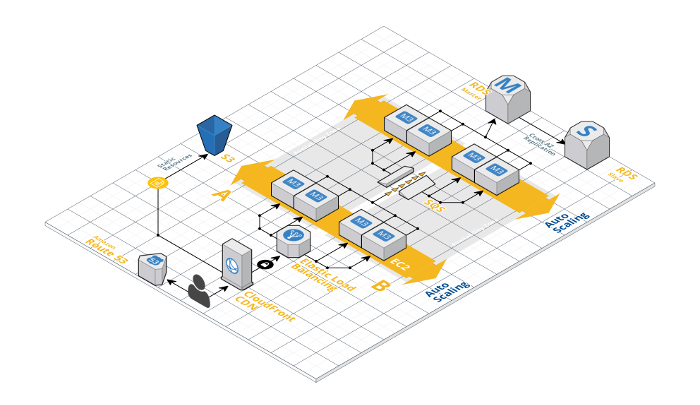
\includegraphics[width=0.8\textwidth]{resources/chapter-2-infrastructure-diagram.png}
        \caption{Contoh gambar}
    \end{figure}

    \subsubsection{Subsubbab}

    \blindtext

\section{Studi Terkait}
\blindtext

    %--------------------------------------------------------------------%
%
% Bab III — Analisis dan Perancangan
%
% @author Petra Novandi
%
%--------------------------------------------------------------------%
%
% Berisi analisis masalah, solusi umum, dan rancangan solusi.
% Ganti teks placeholder dengan isi sebenarnya.
%
%--------------------------------------------------------------------%

\chapter{Analisis dan Perancangan}

Bab ini menjelaskan bagaimana persoalan yang dirumuskan di Bab I
dianalisis dan dirancang solusinya. Pembaca seharusnya memahami
pendekatan yang diambil serta alasan pemilihan solusi sebelum
membaca bab evaluasi.

\section{Analisis Masalah}

Jelaskan persoalan tugas akhir secara rinci berdasarkan rumusan
masalah. Uraikan kondisi yang ada, kebutuhan pengguna atau sistem,
serta kendala yang menjadi fokus penyelesaian.

\blindtext

\section{Solusi Umum}

Deskripsikan solusi atau pendekatan umum yang relevan dengan
persoalan. Bandingkan alternatif yang ada dan jelaskan mengapa
pendekatan tertentu dipilih untuk dikembangkan lebih lanjut.

\blindtext

\section{Rancangan Solusi}

Uraikan rancangan solusi yang diusulkan, meliputi arsitektur,
komponen, alur kerja, model data, antarmuka, atau aspek teknis
lainnya sesuai topik tugas akhir. Contoh berikut menampilkan data
dari berkas CSV di direktori \texttt{resources/}.

\begin{table}[ht]
    \centering
    \caption{Kebutuhan fungsional sistem}
    \label{tab:sample-requirements}
    \csvautotabular{resources/chapter-3-sample-requirements.csv}
\end{table}

\begin{table}[ht]
    \centering
    \caption{Komponen arsitektur sistem}
    \label{tab:sample-components}
    \csvautotabular{resources/chapter-3-sample-components.csv}
\end{table}

    \subsection{Subbab}

    \blindtext

    \subsubsection{Subsubbab}

    \blindtext

\blindtext

    %--------------------------------------------------------------------%
%
% Bab IV — Evaluasi dan Pembahasan
%
% @author Petra Novandi
%
%--------------------------------------------------------------------%
%
% Berisi tujuan pengujian, skenario, hasil pengujian, dan pembahasan.
% Ganti teks placeholder dengan isi sebenarnya.
%
%--------------------------------------------------------------------%

\chapter{Evaluasi dan Pembahasan}

Bab ini mempresentasikan pengujian solusi yang dirancang pada Bab
III dan membahas apakah tujuan serta rumusan masalah telah
terpenuhi. Hasil yang ditampilkan harus dapat dipertanggungjawabkan
secara objektif.

\section{Tujuan Pengujian}

Tuliskan tujuan pengujian yang spesifik dan terukur. Setiap tujuan
sebaiknya berkaitan langsung dengan tujuan tugas akhir dan
rumusan masalah di Bab I.

\blindtext

\section{Skenario Pengujian}

Jelaskan metode, lingkungan, data uji, dan langkah-langkah
pengujian yang dilakukan. Skenario harus cukup jelas agar pengujian
dapat direplikasi oleh pembaca.

\blindtext

\section{Hasil Pengujian}

Sajikan hasil pengujian secara faktual menggunakan tabel, grafik,
atau angka. Hindari interpretasi panjang di subbab ini; fokuskan
pada data dan temuan yang diperoleh.

    \subsection{Subbab}

    \blindtext

    \subsubsection{Subsubbab}

    \blindtext

\blindtext

\section{Pembahasan}

Interpretasikan hasil pengujian dan kaitkan dengan rumusan masalah
serta tujuan tugas akhir. Jelaskan apakah solusi yang diusulkan
berhasil, keterbatasannya, dan perbandingannya dengan studi terkait
jika relevan.

\blindtext

    %--------------------------------------------------------------------%
%
% Bab V — Penutup
%
% @author Petra Novandi
%
%--------------------------------------------------------------------%
%
% Berisi kesimpulan dan saran. Ganti teks placeholder dengan isi
% sebenarnya.
%
%--------------------------------------------------------------------%

\chapter{Penutup}

Bab ini merangkum hasil tugas akhir dan memberikan saran untuk
pengembangan lebih lanjut. Kesimpulan harus menjawab rumusan masalah
dan tujuan yang telah dirumuskan di awal laporan.

\section{Kesimpulan}

Tuliskan kesimpulan utama berdasarkan hasil analisis, perancangan,
dan evaluasi. Setiap poin kesimpulan sebaiknya merujuk pada tujuan
atau rumusan masalah yang telah diselesaikan.

\blindtext

\section{Saran}

Berikan saran yang konstruktif untuk pengembangan solusi, perbaikan
metodologi, atau penelitian lanjutan. Saran dapat mencakup aspek
teknis, evaluasi, maupun implementasi di lingkungan nyata.

\blindtext


    % Daftar Rujukan (gaya APA)
    \printbibliography[title={DAFTAR RUJUKAN}]
    \addcontentsline{toc}{chapter}{Daftar Rujukan}

    %----------------------------------------------------------------%
    % Lampiran — label "Lampiran <angka>".
    %----------------------------------------------------------------%
    \appendix
    \renewcommand{\thechapter}{\arabic{chapter}}
    \titleformat{\chapter}[display]
      {\normalsize\bfseries\centering}
      {Lampiran\ \thechapter}{0pt}
      {\MakeUppercase}

    \addcontentsline{toc}{chapter}{Lampiran}

    %--------------------------------------------------------------------%
%
% Lampiran A — Instrumen Pengujian
%
% @author Petra Novandi
%
%--------------------------------------------------------------------%
%
% Berisi instrumen atau alat bantu pengujian. Ganti teks placeholder
% dengan isi sebenarnya.
%
%--------------------------------------------------------------------%

\chapter{Instrumen Pengujian}

\blindtext

    %--------------------------------------------------------------------%
%
% Lampiran B — Rincian Kasus Uji
%
% @author Petra Novandi
%
%--------------------------------------------------------------------%
%
% Berisi rincian kasus uji. Ganti teks placeholder dengan isi
% sebenarnya.
%
%--------------------------------------------------------------------%

\chapter{Rincian Kasus Uji}

\blindtext


    %--------------------------------------------------------------------%
%
% Riwayat Hidup (Pedoman UM Lampiran 13) — naratif, spasi tunggal,
% tanpa foto. Batasi pendidikan sampai jenjang di atas SMA.
%
%--------------------------------------------------------------------%

\clearpage
\addcontentsline{toc}{chapter}{Riwayat Hidup}

\begin{center}
    \bfseries RIWAYAT HIDUP
\end{center}

\begin{singlespace}
\blindtext
\end{singlespace}
     % Riwayat Hidup

\end{document}
